\documentclass[10pt,a4paper]{article}
\usepackage[utf8]{inputenc}
\usepackage{amsmath}
\usepackage{amsfonts}
\usepackage{makeidx}
\usepackage{draftwatermark}
\SetWatermarkText{CONFIDENTIAL}
\SetWatermarkScale{4}
\usepackage{listings}
\usepackage{color}

\definecolor{mygreen}{rgb}{0,0.6,0}
\definecolor{mygray}{rgb}{0.5,0.5,0.5}
\definecolor{mymauve}{rgb}{0.58,0,0.82}

\lstset{ %
  backgroundcolor=\color{white},   % choose the background color; you must add \usepackage{color} or \usepackage{xcolor}
  basicstyle=\footnotesize,        % the size of the fonts that are used for the code
  breakatwhitespace=false,         % sets if automatic breaks should only happen at whitespace
  breaklines=true,                 % sets automatic line breaking
  captionpos=b,                    % sets the caption-position to bottom
  commentstyle=\color{mygreen},    % comment style
  deletekeywords={...},            % if you want to delete keywords from the given language
  escapeinside={\%*}{*)},          % if you want to add LaTeX within your code
  extendedchars=true,              % lets you use non-ASCII characters; for 8-bits encodings only, does not work with UTF-8
  frame=single,                    % adds a frame around the code
  keepspaces=true,                 % keeps spaces in text, useful for keeping indentation of code (possibly needs columns=flexible)
  keywordstyle=\color{blue},       % keyword style
  language=Octave,                 % the language of the code
  morekeywords={*,...},            % if you want to add more keywords to the set
  numbers=left,                    % where to put the line-numbers; possible values are (none, left, right)
  numbersep=5pt,                   % how far the line-numbers are from the code
  numberstyle=\tiny\color{mygray}, % the style that is used for the line-numbers
  rulecolor=\color{black},         % if not set, the frame-color may be changed on line-breaks within not-black text (e.g. comments (green here))
  showspaces=false,                % show spaces everywhere adding particular underscores; it overrides 'showstringspaces'
  showstringspaces=false,          % underline spaces within strings only
  showtabs=false,                  % show tabs within strings adding particular underscores
  stepnumber=2,                    % the step between two line-numbers. If it's 1, each line will be numbered
  stringstyle=\color{mymauve},     % string literal style
  tabsize=2,                       % sets default tabsize to 2 spaces
  title=\lstname                   % show the filename of files included with \lstinputlisting; also try caption instead of title
}
\usepackage{amssymb}
\usepackage{graphicx}
\usepackage{float}
\usepackage{hyperref}
%\usepackage[Sonny]{fncychap}
\floatstyle{boxed}
\restylefloat{figure}
\usepackage[left=2cm,right=2cm,top=2cm,bottom=2cm]{geometry}
\newcommand{\HRule}{\rule{\linewidth}{0.5mm}}
\begin{document}
\begin{titlepage}
\begin{center}

% Upper part of the page. The '~' is needed because \\
% only works if a paragraph has started.
%
\includegraphics[width=0.15\textwidth]{./logo}~\\[1cm]

%\textsc{\LARGE University of Beer}\\[1.5cm]

\textsc{\Large Project Proposal}\\[0.5cm]

% Title
\HRule \\[0.4cm]
{ \huge \bfseries Project Quad \\[0.4cm] }

\HRule \\[1.5cm]

% Author and supervisor
\begin{minipage}{0.4\textwidth}
\begin{flushleft} \large
\emph{Author:}\\
Andy \textsc{Fang}
\end{flushleft}
\end{minipage}
\begin{minipage}{0.4\textwidth}
\begin{flushright} \large
\emph{Supervisor:} \\
Dr.~Mark \textsc{Brown}
\end{flushright}
\end{minipage}

\vfill

% Bottom of the page
{\large \today}

\end{center}
\end{titlepage}
%\maketitle
\newpage
\tableofcontents 
\newpage
\section{Basic Concept}
\subsection{Quadcopter}
\subsubsection{Defination}
A quadcopter, also called a quadrotor helicopter, quadrocopter, quadrotor, is a multicopter that is lifted and propelled by four rotors.\cite{cite1}
\begin{figure}[h!]
  
  \centering
    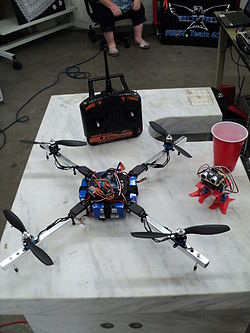
\includegraphics[width=0.3\textwidth]{./Pictures/250px-ReuseumMakerFaireQuadrotor.JPG}
    \caption{A Maker Faire quadcopter in Garden City, Idaho\cite{cite1}}\\
\end{figure}
\subsubsection{Flight Control}
\begin{figure}[h!]
  
  \centering
    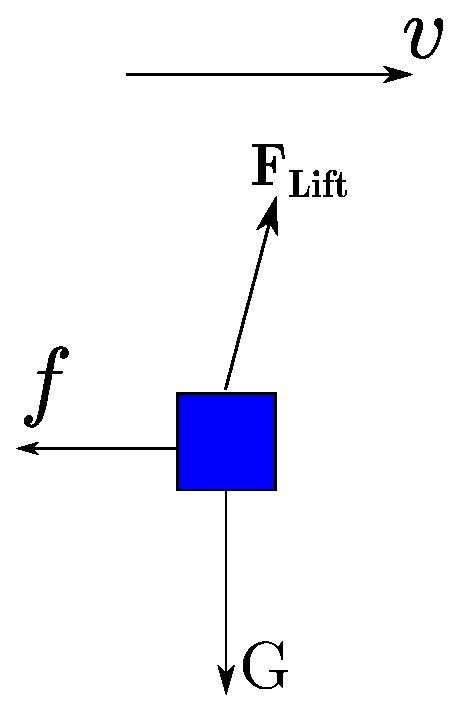
\includegraphics[width=0.3\textwidth]{./Pictures/flying.eps}
    \caption{The forces effected on the quadcopter while making stable movement.}\\
\end{figure}
%\newpage
\textbf{[ Hover ]}
\begin{figure}[H]
  
  \centering
    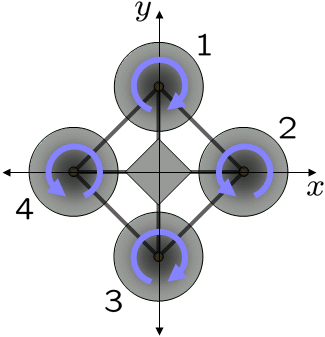
\includegraphics[width=0.3\textwidth]{./Pictures/Quadrotor_yaw_torque.png}
    \caption{The example model of quadcopter.}\\
\end{figure}


Each rotor porduces both thrust and torque. If all the rotors are spining at the same angular velocity, and as the example shows, with rotor 1,3 spining clockwise and rotor 2,4 spining counterclockwise, the angular acceleration on the yaw-axis will be zero. 
This is the method to hovering.

\textbf{[ Yaw ]}\\
\begin{figure}[H]
  
  \centering
    
\includegraphics[width=0.3\textwidth]{./Pictures/yaw.png}
    \caption{Yaw control}
\end{figure}
The method of making yaw control can be done by adjusting the angular velocity of one pair of rotors.\\
\textbf{[ Pitch ]}\\
\begin{figure}[H]
  
  \centering
    
\includegraphics[width=0.3\textwidth]{./Pictures/pitch.png}
    \caption{Pitch control}
\end{figure}
The method of making pitch control can be done by increasing one rotor's spinning velocity and decreasing the opposite rotor's spinning velocity.\\
\textbf{[ Roll ]}\\
\begin{figure}[H]
  
  \centering
    
\includegraphics[width=0.3\textwidth, angle=90]{./Pictures/pitch.png}
    \caption{Roll control}
\end{figure}
The method of making roll control is similar to making pitch control.\\
It can be done by increasing one rotor's spinning velocity and decreasing the opposite rotor's spinning velocity.\\

\textbf{The eeeeeeeeeeasy way}\\
Use the ardupilot\cite{cite2} library.\\
\textbf{The harrrrrrrrrrd way}\\
Write the control system complete from scratch.\\
Which is possible, but might take a loooooooooong time.
\section{Optical Tracking}
\subsection{Overview}
The Optical Tracking System is implemented with three subsystems:
\begin{enumerate}
  \item Video Extraction
  \item Pinhole Camera Model
  \item Epipolar Geometry
\end{enumerate}
\subsection{Video Extraction}
The Video Extraction system's function is to extract the location of a patricular object within the video footage. The objects, in this case, are differently colored small balls. The small balls represent sever key points of the Quadcopter. By determining the location of the balls, we will be able to calculate the position and attitude of the Quadcopter.
The procedure of video extraction is described as following:
\begin{enumerate}
  \item Shotting: Get images from camera,
  \item Transforming: transform the image to HSV colorspace,
  \item Extracting: use tresholding to extract pixels in patricular color range, then use histogram and backprojection to determin the probablity that the pixels belong to the model,
  \item Denoising: use opening and closing to denoise,
  \item Determining: use CamShift algorithm to determin the centroid of the extracted pixels.
\end{enumerate}
\subsubsection{Shooting}
In this project, v4l\footnote{a.k.a. Video For Linux} is as the middleware of OpenCV and camera. With \emph{v4l} and \emph{OpenCV}, reading an image from camera is as easy as following:
\lstset{language=python}
\begin{lstlisting}
cap = cv2.VideoCapture(source)
img = cap.read()
\end{lstlisting}
\subsubsection{Transforming}
Different from the RGB colorspace, HSV colorspace has a unique character: its V channel represents the brightness. If we remove V channel from tresholding, the same color profile will be able to work in different lighting conditions.
The transforming process is described below\cite{cite4}:
\begin{align}
  M &= \operatorname{max}(R, G, B) \\
  m &= \operatorname{min}(R, G, B) \\
  C &= M - m\\
  H^\prime &=
    \begin{cases}
      \mathrm{undefined},        &\mbox{if } C = 0 \\
      \frac{G - B}{C} \;\bmod 6, &\mbox{if } M = R \\
      \frac{B - R}{C} + 2,       &\mbox{if } M = G \\
      \frac{R - G}{C} + 4,       &\mbox{if } M = B
    \end{cases} \\
  H        &= 60^\circ \times H^\prime\\
  V &= M\\
   S &=
    \begin{cases}
      0,           &\mbox{if } C = 0 \\
      \frac{C}{V}, &\mbox{otherwise}
    \end{cases}
\end{align}
The code used to transform the image is:
\begin{lstlisting}
hsv = cv2.cvtColor(img, cv2.COLOR_BGR2HSV)
\end{lstlisting}
Note that by default, OpenCV uses BGR color space.
\subsubsection{Extracting}
OpenCV's built in treshold function is used to utilize multithreading.
The process of tresholding is printed below:
\begin{lstlisting}
mask = cv2.inRange(hsv, np.array((0., 60., 32.)), np.array((180., 255., 255.)))
\end{lstlisting}
However, simply tresholding is often not enough. The object tracked can have a complex color feature. In order to track the entire object, it is necessary to consider all of the features. Histogram is used to model the color distribution of an object, and me can then map the probability of pixels using backprojection.\\
\begin{figure}[h!]

  \centering
    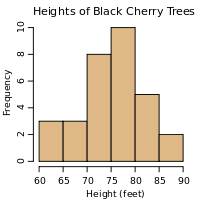
\includegraphics[width=0.2\textwidth]{../Pictures/histogram.JPG}
    \caption{A sample histogram\cite{cite5}}\\
\end{figure}
Backprojection uses the modeled histogram to find the probability that certain pixel belongs to the model. Consider an image matrix $M$, each pixel can be described as pair $(H_{i,j},S_{i,j})$. We can use the two values to create a 2D histogram that represents the distribution of certain color range in $H$ and $S$. Below is a sample 2D histogram generated by \emph{OpenCV Python Sample}.\\
\begin{figure}[h!]

  \centering
    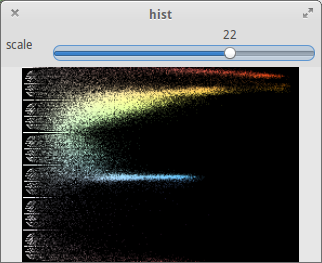
\includegraphics[width=0.3\textwidth]{../Pictures/2dhist.png}
    \caption{A sample 2D histogram}\\
\end{figure}
After generating the histogram, the probability that a pixel belongs to the model can be expressed by the following steps:
\begin{enumerate}
  \item Find the pair $(H_{i,j},S_{i,j})$ of a pixel,
  \item find the correspondent bin in the histogram,
  \item get the relative frequency of the bin.
\end{enumerate}
Then we can use the frequency to map a binary image. In this image, each pixel represents the probability that the correspondent pixel in the original image belongs to the model. Below is an example backproject image:\\
\begin{figure}[h!]

  \centering
    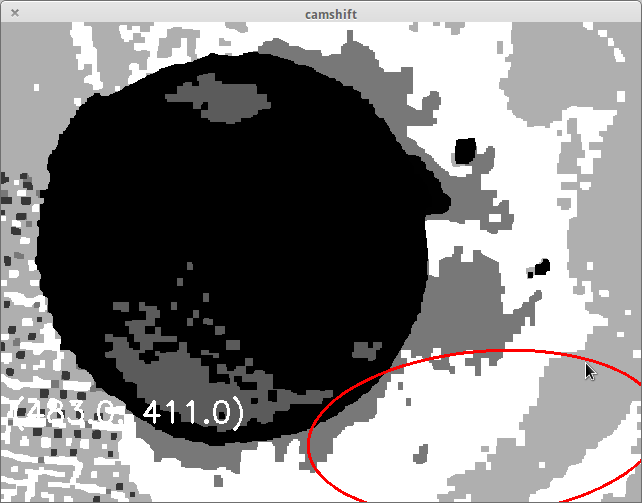
\includegraphics[width=0.5\textwidth]{../Pictures/backproject.png}
    \caption{A sample backprojrction}\\
\end{figure}
\subsubsection{Denoising}
After calculating the backproject image, we will be able to use morphology transformation to remove noises. In this projcet, we used Opening and Closing to remove small noise pixels and fill black pixel holes in the backprojection.\\
\begin{figure}[h!]

  \centering
    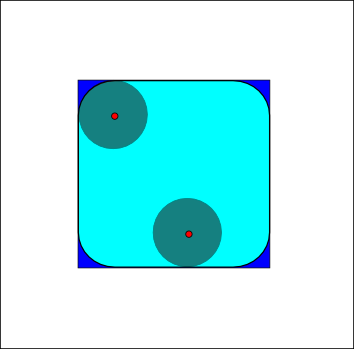
\includegraphics[width=0.3\textwidth]{../Pictures/Opening.png}
    \caption{Sample Opening operation\cite{cite7}}\\
\end{figure}
\begin{figure}[h!]

  \centering
    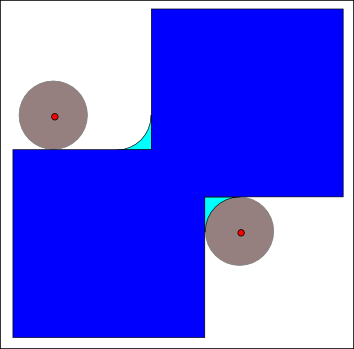
\includegraphics[width=0.3\textwidth]{../Pictures/Closing.png}
    \caption{Sample Closing operation\cite{cite6}}\\
\end{figure}

The result is significant. A great deal of noises is removed in this process:\\
\begin{figure}[h!]

  \centering
    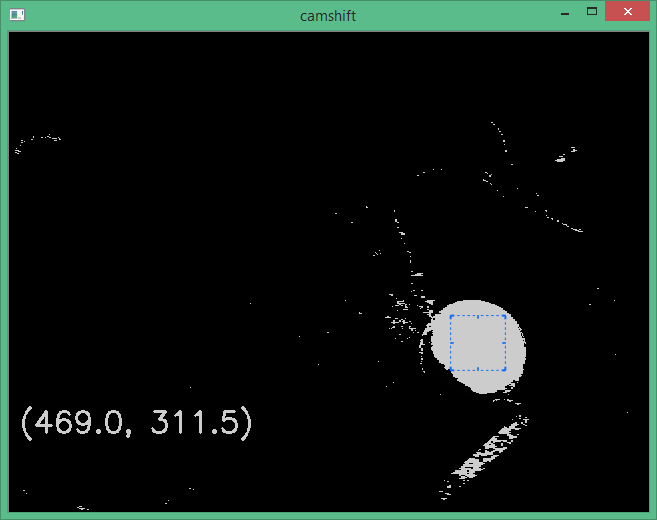
\includegraphics[width=0.3\textwidth]{../Pictures/before.png}
    \caption{Befor morphology transformation}\\
\end{figure}
\begin{figure}[h!]

  \centering
    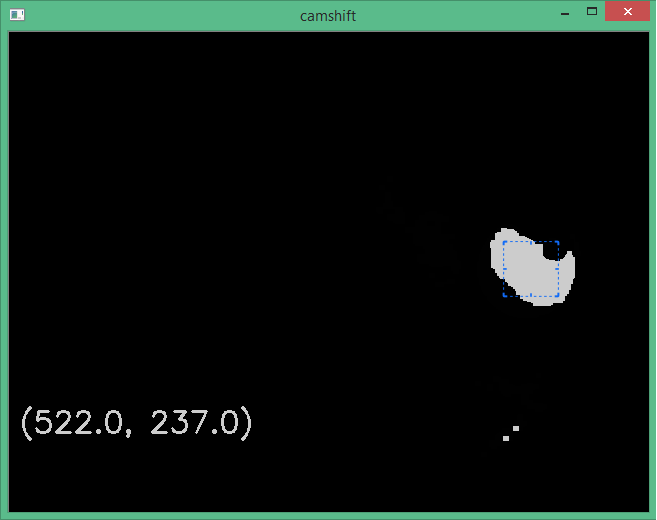
\includegraphics[width=0.3\textwidth]{../Pictures/after.png}
    \caption{After morphology transformation}\\
\end{figure}

\newpage

\begin{thebibliography}{9}

\bibitem{cite1}
  Wikipedia ,
  \emph{Quadcopter}.
  \url{https://en.wikipedia.org/wiki/Quadcopter}
\bibitem{cite2}
  GitHub ,
  \emph{ardupilot}.
  \url{https://github.com/diydrones/ardupilot},\url{http://ardupilot.com/}

\end{thebibliography}




\end{document}